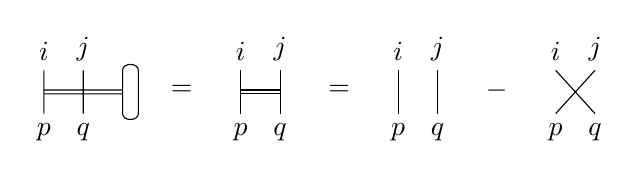
\begin{tikzpicture}
    \coordinate(origin1)at(-.5,0);
    \node at(1.25,-.255)[anchor=center]{$=$};
    \coordinate(origin2)at(2,0);
    \node at(3.25,-.255)[anchor=center]{$=$};
    \coordinate(origin3)at(4,0);
    \node at(5.25,-.255)[anchor=center]{$-$};
    \coordinate(origin4)at(6,0);
    \draw
    (origin1)node[anchor=south]{$i$}
    --++(0,-.55)node[anchor=north]{$p$}
    ++(.5,.55)node[anchor=south]{$j$}
    --++(0,-.55)node[anchor=north]{$q$}
    ++(.5,.55)node[anchor=south](k){}
    --++(0,-.55)node[anchor=north](r){}
    ++(0,.25)--++(-1,0)
    ++(0,.05)--++(1,0)
    (k.south) .. controls ++(0,.1) and ++(0,.1) .. ++(.2,0)
    --++(0,-.55)
    .. controls ++(0,-.1) and ++(0,-.1) .. +(-.2,0)
    ;
    \draw
    (origin2)node[anchor=south]{$i$}
    --++(0,-.55)node[anchor=north]{$p$}
    ++(.5,.55)node[anchor=south]{$j$}
    --++(0,-.55)node[anchor=north]{$q$}
    ++(0,.25)--++(-.5,0)
    ++(0,.05)--++(.5,0)
    ;
    \draw
    (origin3)node[anchor=south](i){$i$}
    ++(.5,0)node[anchor=south](j){$j$}
    ++(-.5,-.55)node[anchor=north](p){$p$}
    ++(.5,0)node[anchor=north](q){$q$}
    (i.south)--(p.north)
    (j.south)--(q.north)
    ;
    \draw
    (origin4)node[anchor=south](i){$i$}
    ++(.5,0)node[anchor=south](j){$j$}
    ++(-.5,-.55)node[anchor=north](p){$p$}
    ++(.5,0)node[anchor=north](q){$q$}
    (i.south)--(q.north)
    (j.south)--(p.north)
    ;
\end{tikzpicture}
